\documentclass{article}

\usepackage[margin=1in]{geometry}
\usepackage{lipsum}
\usepackage{graphicx}
\usepackage{amsmath}

\begin{document}
    \title{Introduction to Mathematical Proofs}
    \author{Charles E. Roberts}
    \maketitle

    \tableofcontents

    \section{Set Theory}

    \subsection{definition of subset}

    Let $A$ and $B$ be sets. $A$ is a subset of $B$, written $A \subseteq B$, if and only if every element of $A$ is an element of $B$. Symbolically,
    \begin{equation}
    A \subseteq B \Leftrightarrow (\forall x)[(x \in A) \Rightarrow (x \in B)]
    \end{equation}

    \subsection{equality of sets}
    
    Two sets are equal, written $A = B$, if and only if they are identical sets, that is, if and only if they have exactly the same elements.
    \begin{equation}
    \begin{aligned}
    & A = B \Leftrightarrow (\forall x)[(x \in A) \Leftrightarrow (x \in B)] \\
    & (\forall x)[[(x \in A) \Rightarrow (x \in B)] \wedge [(x \in B) \Rightarrow (x \in A)]] \\
    & [(\forall x)[(x \in A) \Rightarrow (x \in B)]] \wedge [(\forall x)[(x \in B) \Rightarrow (x \in A)]]
    \end{aligned}
    \end{equation}
    which is $A \subseteq B$ and $B \subseteq A$, we define \textbf{equality of sets} as follows.
   
    Let $A$ and $B$ be sets. Then $A = B \Leftrightarrow [(A \subseteq B) \wedge (B \subseteq A)]$. Example: $A = \{1,2,3\}$ and $B = \{3,1,2,2,1\}$.

    \subsection{proper subset}

    The set $A$ is a \textbf{proper subset} of the set $B$, written $A \subset B$, if and only if $A$ is a subset of $B$ and $A \neq B$. Symbolically,
    \begin{equation}
    A \subset B \Leftrightarrow [(A \subseteq B) \wedge (A \neq B)].
    \end{equation}
    A is a proper subset of $B$ provided every element of $A$ is an element of $B$ and there exists at least one element of $B$ which is not an element of $A$.

    \subsection{power set}

    Let $A = \{ a_1,a_2,...,a_n\}$ be a set with $n \geq 1$ elements. In creating a subset $X$ of $A$ there are $n$ decisions to be made --- namely, whether $a_i \in X$ or $a_i \notin X$ for $i = 1,2,...,n$. Since there are $n$ decisions to be made and two possible choices for each decision, there is a total of $2^n$ possible subsets $X$ of $A$. \\
    \\
    \textbf{Example:}
    \begin{enumerate} 
    \item The two subsets of the set $\{1\}$ are $\emptyset$ and $\{1\}$
    \item The eight subsets of the set $\{ x,y,z\}$ are the sets $\emptyset, \{ x \}, \{ y \}, \{ z \},\{x,y\},\{x,z\},\{y,z\}$, and $\{x,y,z\}$
    \end{enumerate}

    The set of all subsets of a finite set $A$ is denoted by $P(A)$ and is called the \textbf{power set} of $A$. The name power set comes from the fact that if the set $A$ has $n$ elements, then its power set $P(A)$ has $2^n$ elements.

    \subsection{universe}

    At the beginning of a particular discussion a set called the \textbf{universe} is specified. The universe need not be the same set for all discussions, in one discussion the universe might be the set of integers, in another discussion the universe might be the set of all triangles, etc.

    \subsection{union}

    The set $A$ union $B$ is the subset of $U$ which contains all elements that belong either to $A$ or to $B$ or to both $A$ and $B$. The set $A$ union $B$ is denoted by $A \cup B$.
    \begin{equation}
    A \cup B = \{x | x \in A \textrm{ or } x \in B \} = \{x | (x \in A) \vee (x \in B)\}
    \end{equation}
    For example, if the universe is the set of natural numbers, $A = \{1,3,5,7\}$, and $B = \{2,4,6\}$, then $A \cup B = \{1,2,3,4,5,6,7\}$.
    \begin{figure}[h]
    \centering
    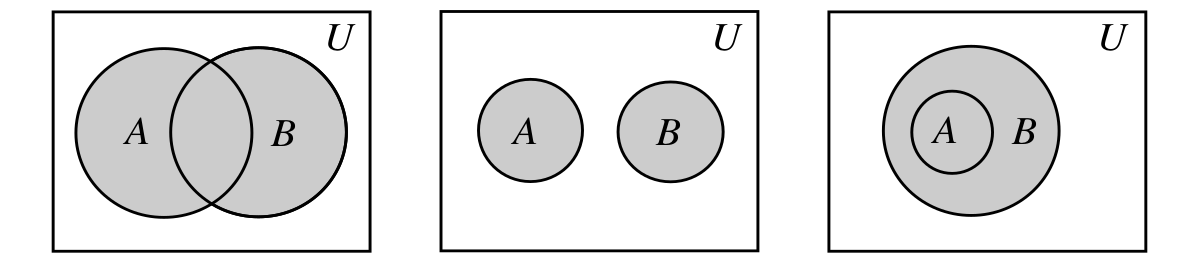
\includegraphics[width=0.5\textwidth]{./images/set-theory-1}
    \caption{Three Venn diagrams for $A \cup B$}
    \end{figure}

    \subsection{intersect}

    The set $A$ intersect $B$ is the subset of $U$ which contains all elements that belong to both $A$ and $B$. The set $A$ intersect $B$ is denoted by $A \cap B$.
    \begin{equation}
    A \cap B = \{x | x \in A \textrm{ and } x \in B\} = \{x|(x \in A) \wedge (x \in B)\}.
    \end{equation}
    For example, if the universe is the set of integers, $A = \{-2,-1,0,1,2\}$, and $B = \{-4,-2,0,2\}$, then $A \cap B = \{-2,0,2\}$. When $A \cap B = \emptyset$, the sets $A$ and $B$ are said to be disjoint.
    \begin{figure}[h]
    \centering
    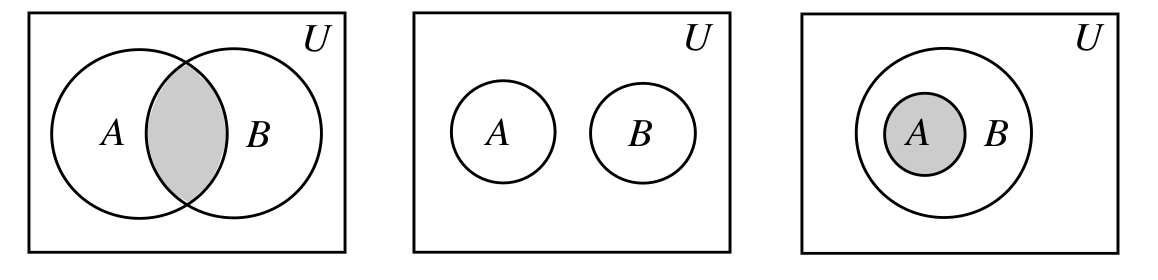
\includegraphics[width=0.5\textwidth]{./images/set-theory-2}
    \caption{Three Venn diagrams for $A \cap B$}
    \end{figure}
    
    \subsection{complement}

    The complement of the set $A$, written $A'$, is the set of all elements in the universe, $U$, which are not in the set $A$. Hence,
    \begin{equation}
    A' = \{x | x \in U \textrm{ and } x \notin A\} = \{x | (x \in U) \wedge (x \notin A) \}
    \end{equation}
    For example, if the universe $U = \{1,2,3,4,5\}$ and $A = \{2,4\}$, then $A' = \{1,3,5\}$
    \begin{figure}[h]
    \centering
    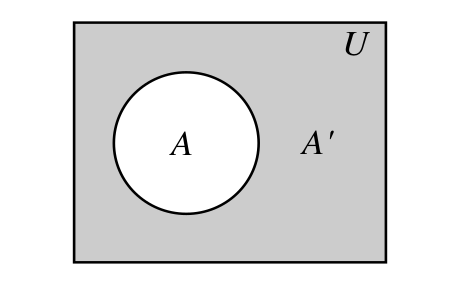
\includegraphics[width=0.5\textwidth]{./images/set-theory-3}
    \caption{A Venn diagram of $A$ and its complement $A'$.}
    \end{figure}

    \subsection{dual of sets and principle of duality for set theory}

    An equation, expression, or statemente in set theory which is obtained by interchanging $\cup$ and $\cap$ and interchanging the sets $\emptyset$ and $U$ is called the \textbf{dual} of the equation, expression, or statement accordingly. Hence, the dual of the statement $A \cup B = B \cup A$ is the statement $A \cap B = B \cap A$. Likewise, the dual of the statement $A \cup \emptyset = A$ is the statement $A \cap U = A$.

    The principle of duality for set theory says "If $T$ is a theorem which is written in terms of $\cup,\cap$ and $'$, then the dual statement $T^D$ is also a theorem". Since we have proven $A \cup B = B \cup A$ is a theorem of set theory, by the principle of duality, $A \cap B = B \cap A$ is a theorem of set theory also.

    \subsection{set difference of $A$ and $B$}
    Let $A$ and $B$ be two subsets of the universe $U$. The set difference of $A$ and $B$, written $A - B$, is the set of all elements in the set $A$ that are not in the set $B$:
    $$
    A - B = \{x | x \in A \textrm{ and } x \notin B\} = \{x | (x \in A) \wedge (x \notin B) \}
    $$
    For example, if the universe is the set of natural numbers, $A = \{3,5,7,8\}$, and $B = \{1,3,7,9\}$, then $A - B = \{5,8\}$ and $B - A = \{1,9\}$.

    Let $A$ and $B$ be subsets of the universal set $U$. Then $A - B = A \cap B'$.
    $$
    \begin{aligned}
    x \in A \cap B^{\prime} & \Leftrightarrow(x \in A) \wedge\left(x \in B^{\prime}\right) & & \text { Definition of } A \cap B^{\prime} \\
    & \Leftrightarrow(x \in A) \wedge[(x \in U) \wedge(x \notin B)] & & \text { Definition of } B^{\prime} \\
    & \Leftrightarrow[(x \in A) \wedge(x \in U)] \wedge(x \notin B) & & \text { Associative law of conjunction } \\
    & \Leftrightarrow[x \in(A \cap U)] \wedge(x \notin B) & & \text { Definition of } A \cap U \\
    & \Leftrightarrow(x \in A) \wedge(x \notin B) & & \text { Substitution } A \cap U=A \\
    & \Leftrightarrow x \in A-B & & \text { Definition of } A-B \\
    \text { Thus, }(\forall x \in&U)\left[\left(x \in\left(A \cap B^{\prime}\right)\right) \Leftrightarrow(x \in(A-B))\right] . & \text { Hence, } A-B=A \cap B^{\prime}.
    \end{aligned}
    $$
    This theorem shows how to write the set $A - B$ in terms of set intersection and set complementation. Thus, to prove theorems which involve the difference of two sets, we may write the difference of sets in terms of set intersection and complementation and then use the algebra of sets to prove the desired result.

    \subsection{ordered pair, ordered n-tuple}

    By an ordered pair we mean an entity consisting of two elements in a specific order. We denote the ordered pair with $a$ as first element and $b$ as second element by $(a,b)$.
    $$
    (a,b) = \{\{a\},\{a,b\}\}.
    $$
    \textbf{Theorem}: The ordered pair $(a,b) = (c,d)$ if and only if $a = c$ and $b = d$.

    Generalizing the concept of an ordered pair, we define an ordered triple to be an entity consisting of three elements in a specific order such as $(a,b,c)$ in which $a$ is the first element, $b$ is the second element, and $c$ is the third element. Two ordered triples $(a,b,c)$ and $(x,y,z)$ are equal if and only if $a = x$ and $b = y$ and $c = z$.

    An ordered n-tuple is denoted by $(a_1,a_2,...,a_n)$ and $(a_1,a_2,...,a_n) = (b_1,b_2,...,b_n)$ if and only if $a_i = b_i$ for $i = 1,2,...,n$.

    \subsection{Cartesian product of $A$ and $B$}

    The Cartesian product of $A$ and $B$, written as $A \times B$, is the set of all ordered pairs $(a,b)$ such that $a \in A$ and $b \in B$.
    $$
    A \times B = \{(a,b) | a \in A \textrm{ and } b \in B\}.
    $$
    If $(a,b) \in A \times B$, then it must be true that $a \in A$ and $b \in B$, whereas, if $(a,b) \notin A \times B$, then either $a \notin A$ or $b \notin B$.

    As an example, let $A=\{1, a, \#\}$ and $B=\{\$, @\}$; then
    $$
    A \times B=\{(1, \$),(1, @),(a, \$),(a, @),(\#, \$),(\#, @)\}
    $$
    and
    $$
    B \times A=\{(\$, 1),(\$, a),(\$, \#),(@, 1),(@, a),(@, \#)\} .
    $$
    As this example illustrates, in general, $A \times B \neq B \times A$. That is, the Cartesian product is not commutative. Let $A$ be a finite set with $m$ elements and let $B$ be a finite set with $n$ elements, then the Cartesian products $A \times B$ and $B \times A$ both have $mn$ elements which are ordered pairs.

    \subsection{intervals as subsets of real numbers}

    We can define subsets of the real numbers which are intervals using inequalities as follows: Let $a, b \in \mathbf{R}$ and let $a<b$. \\
    The \textbf{open interval} $(a, b)$ is the subset of the real numbers
    $$
    (a, b)=\{x \in \mathbf{R} \mid a<x<b\} .
    $$
    The \textbf{closed interval} $[a, b]$ is the subset of the real numbers
    $$
    [a, b]=\{x \in \mathbf{R} \mid a \leq x \leq b\} .
    $$
    The \textbf{half-open (half-closed) intervals} are
    $$
    [a, b)=\{x \in \mathbf{R} \mid a \leq x<b\}
    $$
    and
    $$
    (a, b]=\{x \in \mathbf{R} \mid a<x \leq b\} .
    $$
    Let $a, b \in \mathbf{R}$ and let $a<b$. The infinite intervals are
    $$
    \begin{aligned}
    {[a, \infty) } &=\{x \in \mathbf{R} \mid a \leq x\} \\
    (a, \infty) &=\{x \in \mathbf{R} \mid a<x\} \\
    (-\infty, b] &=\{x \in \mathbf{R} \mid x \leq b\} \\
    (-\infty, b) &=\{x \in \mathbf{R} \mid x<b\} \\
    (-\infty, \infty) &=\mathbf{R} .
    \end{aligned}
    $$

    \subsection{generalized set union and intersection}

    Let $A_1, A_2$ and $A_3$ be subsets of the universe $U$. The associative law for set union is $(A_1 \cup A_2) \cup A_3 = A_1 \cup (A_2 \cup A_3)$. Essentially, the associative law says we may omit the parentheses and simply write $A_1 \cup A_2 \cup A_3$. Likewise, the set $((A_1 \cup A_2) \cup A_3) \cup A_4$ may be written as $A_1 \cup A_2 \cup A_3 \cup A_4$ and, in general, for $n \in N$ we may write $A_1 \cup A_2 \cup \cdot \cdot \cdot A_n$ without parentheses and without ambiguity. Note that for $n \in N, x \in A_1 \cup A_2 \cup \cdot \cdot \cdot \cup A_n$ if and only if $x \in A_i$ for some $i = 1,2,...n.$

    The \textbf{finite union of the sets} $A_1,A_2,...,A_n$ is
    $$
    \begin{aligned}
    A_1 \cup A_2 \cup \cdot \cdot \cdot \cup A_n & = \{x \in U | x \in A_i \textrm{ for some } i = 1,2,...,n\} \\
    & = \{x \in U | (\exists i \in \{1,2,...,n\})(x \in A_i)\}
    \end{aligned}
    $$
    or
    $$
    \bigcup_{i=1}^{n} A_{i}=A_{1} \cup A_{2} \cup \cdots \cup A_{n}
    $$

    The \textbf{infinite union of the sets} $A_1,A_2,...$ is 
    $$
    \bigcup_{i=1}^{\infty} A_i = A_1 \cup A_2 \cup \cdots = \{x \in U | (\exists i \in N)(x \in A_i)\}
    $$

    The \textbf{finite intersection of the sets} $A_1,A_2,\dots,A_n$ is
    $$
    \begin{aligned}
    \bigcap_{i=1}^{n} A_{i} &=A_{1} \cap A_{2} \cap \cdots \cap A_{n} \\
    &=\left\{x \in U \mid x \in A_{i} \text { for all } i=1,2, \ldots, n\right\} \\
    &=\left\{x \in U \mid(\forall i \in\{1,2, \ldots, n\})\left(x \in A_{i}\right)\right\} .
    \end{aligned}
    $$
    
    The \textbf{infinite intersection of the sets} $A_1,A_2,\dots$ is
    $$
    \bigcap_{i=1}^\infty A_i = A_1 \cap A_2 \cap \cdots = \{x \in U | (\forall i \in N)(x \in A_i)\}
    $$

    \subsection{family of sets}

    A set of sets is often called a family of sets, or simply a family. For instance, the family $\mathcal{A}=\{\{a\},\{a, b\},\{a, b, c\},\{a, b, c, d\}\}$ is a family with four sets and the family $\mathcal{B}=\{(-a, a) \mid a \in(0, \infty)\}$ is an infinite family of open intervals. The union and intersection of a family of sets is defined as follows.

    Let $\mathcal{F}$ be a family of sets which are all subsets of a universe $U$. The union over $\mathcal{F}$ is
    $$
    \bigcup_{A \in \mathcal{F}} A=\{x \in U \mid(\exists A \in \mathcal{F})(x \in A)\} .
    $$

    The intersection over $\mathcal{F}$ is
    $$
    \bigcap_{A \in \mathcal{F}} A=\{x \in U \mid(\forall A \in \mathcal{F})(x \in A)\} .
    $$
    
    \subsection{indexing set}

    Let $\mathcal{F}$ be a nonempty family of sets and let $I$ be a nonempty set with the property that for each $i \in I$ there corresponds a set $A_i \in \mathcal{F}$. Then the family of sets $\mathcal{F} = \{A_i | i \in I\}$ is called an \textbf{indexed family of sets}. The set $I$ is called the \textbf{indexing set} and each $i \in I$ is called an index. \\
    For example, $A_i = [i,i+1)$ are the members of the family of sets $\mathcal{F}$, the natural numbers $N$ is the indexing set $I$, and each natural number $i$ is an index. The family $\mathcal{A} = \{\{a\},\{a,b\},\{a,b,c\},\{a,b,c,d\}\}$ contains four sets and may be indexed by the indexing set $I = \{1,2,3,4\}$ where 1 is associated with the set $\{a\}$, 2 is associated with the set $\{a,b\}$, 3 is associated with the set $\{a,b,c\}$ and 4 is associated with the set $\{a,b,c,d\}$.

    When $\mathcal{F}$ is a nonempty family of sets indexed by the set $I$, the following alternate definitions may be used for $\bigcup_{A \in \mathcal{F}} A$ and $\bigcap_{A \in \mathcal{F}} A$, respectively.
    $$
    \bigcup_{i \in I} A_i = \{x \in U | (\exists i \in I)(x \in A_i)\}
    $$
    and
    $$
    \bigcap_{i \in I} A_i = \{x \in U | (\forall i \in I)(x \in A_i)\}
    $$

    \textbf{Example 3.4.3} Let $\mathcal{F}$ be the empty family of subsets of the natural numbers, $\mathbf{N}$. Show that \\
    $$
    \begin{aligned}
    \bigcap_{A \in \mathcal{F}} A=\mathbf{N},& & \bigcup_{A \in \mathcal{F}} A=\emptyset, & \quad \textrm{ and } & \bigcap_{A \in \mathcal{F}} A \bigcup_{A \in \mathcal{F}} A
    \end{aligned}
    $$

    \textbf{Solution} \\
    a. The statement $(\forall A \in \mathcal{F})(x \in A)$ is equivalent to $(\forall A)[(A \in \mathcal{F}) \Rightarrow$ $(x \in A)]$. Since $\mathcal{F}$ is assumed to be the empty set, the hypothesis of the last statement, $A \in \mathcal{F}$, is false. Consequently, the implication $[(A \in \mathcal{F}) \Rightarrow(x \in A)]$ is true for all $x \in \mathbf{N}$. Hence, $\bigcap_{A \in \mathcal{F}} A=\mathbf{N}$. \\
    b. The statement $(\exists A \in \mathcal{F})(x \in A)$ is logically equivalent to the statement $(\exists A)[(A \in \mathcal{F}) \wedge(x \in A)]$. The negation of the last statement is
    $$
    (\forall A)[\neg(A \in \mathcal{F}) \vee(\neg(x \in A))] \equiv(\forall A)[(A \in \mathcal{F}) \Rightarrow(x \notin A)] .
    $$
    Since $\mathcal{F}=\emptyset, A \in \mathcal{F}$ is false, and the implication $(A \in \mathcal{F}) \Rightarrow(x \notin A)$ is true. Thus, it follows from the definition of union for a family of sets that for $\mathcal{F}=\emptyset, \bigcup_{A \in \mathcal{F}} A=\emptyset$.

    \section{Relations}

    A relation from $A$ to $B$ is any subset of $A \times B$. In particular, when $B = A$, a relation $R$ (the set of ordered pairs which satisfies the relation) from $A$ to $A$ is called a relation on $A$.

    The domain of a relation $R$ from $A$ to $B$ is the set 
    $$
    Dom(R) = \{x \in A | (\exists y \in B)((x,y) \in R)\}. 
    $$ 

    The range of a relation $R$ from $A$ to $B$ is the set
    $$
    Rng(R) = \{y \in B | (\exists x \in A)((x,y) \in R)\}.
    $$

    The domain of a relation $R$ from $A$ to $B$ is the set of all first coordinates of the ordered pairs in the set $R$ and, by definition, the domain of $R$ is a subset of $A$ --- that is, $Dom(R) \subseteq A$. The range of a relation $R$ from $A$ to $B$  is the set of all second coordinates of the ordered pairs in the set $R$ and, by definition, $Rng(R) \subseteq B$.

    Let $R$ be any set of ordered pairs, let $A$ be any set such that $Dom(R) \subseteq A$, and let $B$ be any set such that $Rng(R) \subseteq B$. Then by definition $R$ is a relation from $A$ to $B$. Consequently, every set of ordered pairs is a relation. For example, let $R = \{(1,a),(b,2),(1,2)\}$. Then $Dom(R) = \{1,b\},Rng(R) = \{a,2\},$ and $R$ is a relation from $A = Dom(R)$ to $B = Rng(R)$.

    \subsection{inverse relation}

    Let $S = \{(x,y) \in A \times B | x < y\}$ where $A = \{1,2,3\}$ and $B = \{2,3,4\}$. If we interchange the components of the ordered pairs in the relation $S$, we obtain the set $\{(2, 1), (3, 1), (4, 1), (3, 2), (4, 2), (4, 3)\}$. This relation is designated by $S^{-1}$ and is called the inverse relation of $S$. Observe that Dom($S^{-1}$) = \{2,3,4\} = Rng($S$) and Rng($S^{-1}$) = \{1,2,3\} = Dom($S$).

    In set-builder notation, $S = \{(x,y) \in A \times B | x < y\}$ and the inverse relation $S^{-1} = \{(x,y) \in B \times A | y < x\}$. Thus, if a relation is defined by some condition on the variables $x$ and $y$, then the condition which defines the inverse relation is obtained from the original condition by interchanging the variables $x$ and $y$. If $R$ is a relation from $A$ to $B$, then the inverse relation from $B$ to $A$ is the relation
    $$
    R^{-1} = \{(x,y) \in B \times A | (y,x) \in R\}.
    $$

    \subsection{identity relation}

    An important family of relations is the family of identity relations --- one relation for each nonempty set $A$. This family is defined as follows. Let $A$ be a nonempty set. The identity relation on $A$ is the set
    $$
    I_A = \{(x,x) \in A \times A | x \in A\}.
    $$

    \subsection{equality of relations}

    Let $R$ be a relation from $A$ to $B$ and let $S$ be a relation from $C$ to $D$. The relation $R$ equals $S$, which is denoted by $R = S$, if and only if $A = C, B = D$, and $[(x,y) \in R \Leftrightarrow (x,y) \in S]$. Let $A = \{1,2\} = C, B = \{a,b\} = D, R = \{(1,a),(2,b)\}$ and $S = \{(1,b),(2,a)\}$. Then Dom($R$) = \{1,2\} = Dom($S$) and Rng($R$) = $\{a,b\}$ = Rng($S$); however, $R \neq S$ because $(1,a) \in R$ but $(1,a) \notin S$.
    
    \subsection{composition of relations}

    Let $R$ be a relation from $A$ to $B$ and let $S$ be a relation from $B$ to $C$. The composition of $S$ and $R$ is the relation
    $$
    S \circ R = \{(a,c) \in A \times C | (\exists b \in B)[((a,b) \in R) \wedge ((b,c) \in S)]\}.
    $$
    \textbf{Example} Let $A = \{a,b,c,d\}, B = \{1,2,3,4,5\}, C = \{w,x,y,z\}, R = \{(a,1),(a,2),(b,2),(c,3)\}$, and $S = \{(1,x),(2,y),(4,w)\}$
    $$
    S \circ R = \{(a,x),(a,y),(b,y)\}.
    $$
    Hence, Dom($S \circ R$) = $\{a,b\} \subset A$ and Rng($S \circ R$) = $\{x,y\} \subset C$.
    \begin{figure}[h]
    \centering
    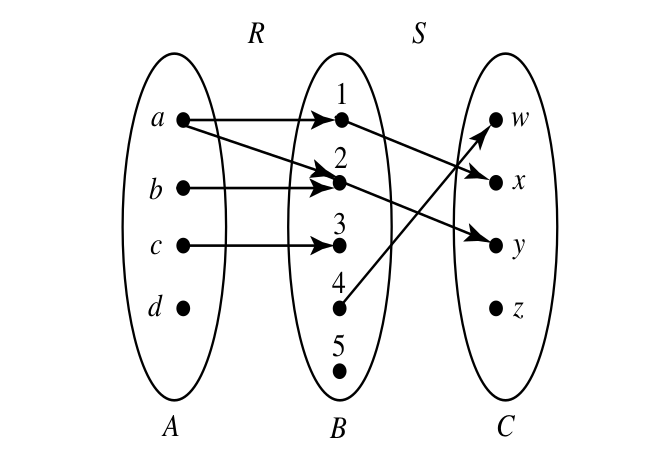
\includegraphics[width=0.5\linewidth]{images/relations-1}
    \caption{Arrow diagram for $S \circ R$}
    \end{figure}
    \newpage
    The binary operation of composition is not commutative. Let $A = \{1,b\}, R = \{(1,b)\}$, and $S = \{(b,1)\}$. Then $S \circ R = \{(1,1)\}, R \circ S = \{(b,b)\}$, and $S \circ R \neq R \circ S$.

    \textbf{Theorem} Let $R$ be a relation from $A$ to $B$, then
    $$
    I_B \circ R = R \textrm{ and } R \circ I_A = R
    $$
    Assume $(x,y) \in R$. Then $y \in B$ and $(y,y) \in I_B$. By the definition of composition, since $(x,y) \in R$ and $(y,y) \in I_B$, it follows that $(x,y) \in I_B \circ R$. Hence, $R \subseteq I_B \circ R$.

    Now assume $(x,y) \in I_B \circ R$. By definition of $I_B \circ R$ there exists a $b \in B$ such that $(x,b) \in R$ and $(b,y) \in I_B$. Since $(b,y) \in I_B, b = y$ and since $(x,b) \in R, (x,y) \in R$. Thus, $I_B \circ R \subseteq R$. Consequently, $I_B \circ R = R$.

    In the following example, we illustrate how to specify the composition of two relations when they are both written in set-builder notation (instead of roster notation). \\
    \\
    Let $T = \{(x,y) \in \mathbf{R} \times \mathbf{R} | x^2 + y^2 = 4\}$ and let $V = \{(x,y) \in \mathbf{R} \times \mathbf{R} | x^2 + (y - 2)^2 = 9\}$.
    $$
    \begin{aligned}
    V \circ T \\
    & = \{(x,y) \in Dom(T) \times Rng(V) | (\exists z \in Rng(T))[((x,z) \in T) \wedge ((z,y) \in V)]\} \\
    & = \{(x,y) \in [-2,2] \times [-1,5] | (\exists z \in [-2,2])[(x^2 + z^2 = 4) \wedge (z^2 + (y - 2)^2 = 9)]\} \\
    & = \{(x,y) \in [-2,2] \times [-1,5] | 4 - x^2 + (y - 2)^2 = 9\} \\
    & = \{(x,y) \in [-2,2] \times [-1,5] | (y - 2)^2 - x^2 = 5\} 
    \end{aligned}
    $$

    \subsection{order relations $<,\leq,>,\geq$}
    
    A set of numbers $S$ is ordered if there exists a subset of positive numbers $S_p$ which satisfy the axioms:

    \begin{enumerate}
    \item (Trichotomy Law) For all $x \in S$ exactly one of the following three statements is true: $x = 0, x \in S_p, -x \in S_p$
    \item For all $x,y \in S_p, x + y \in S_p$
    \item For all $x,y \in S_p, x \cdot y \in S_p$
    \end{enumerate}

    We define negative (positiveness is an undefined concept), $<,\leq,>,\geq$ as follows:
    
    \begin{enumerate}
    \item the order relation $<$ is defined by $x < y \Leftrightarrow y - x$ is positive.
    \item the order relation $>$ is defined by $x > y \Leftrightarrow x - y$ is positive.
    \item the order relation $\leq$ is defined by $x \leq y \Leftrightarrow x < y$ or $x = y$.
    \item the order relation $\geq$ is defined by $x \geq y \Leftrightarrow x > y$ or $x = y$.
    \end{enumerate}
\end{document}
